\chapter{Einleitung}
\thispagestyle{fancy}
\label{chap:Einleitung}
\pagenumbering{arabic}

\noindent
Die \ac{ATS} ist dem Bereich des \ac{NLP} zuzuordnen und gewinnt zunehmend an wissenschaftlicher Relevanz. Obgleich entsprechende Modelle mittlerweile nicht mehr völlig neuartig sind, weisen die Entwicklungen der vergangenen Jahre qualitativ noch viele Potenziale auf \cite[S.~1-2]{YAN19}. Einsatzmöglichkeiten entsprechender \ac{ATS}-Modelle sind beispielsweise die Zusammenfassung von Nachrichten, die Zusammenfassung von Gesprächsprotokollen oder auch die Generierung von Überschriften, um nur wenige zu nennen \cite{GON20}. Ziel ist in jedem Fall die Verdichtung von Informationen und die Reduktion der Lesezeit, wie \autoref{pic:SummarizationProcess} demonstriert.\\

\begin{figure}[h]
  \centering
  \fbox{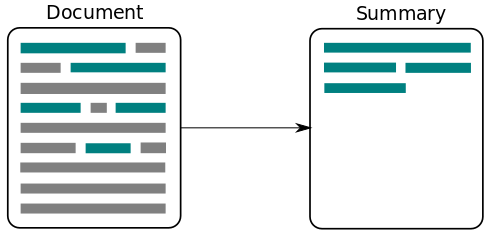
\includegraphics[width=0.6\linewidth]{./source/images/summarizationprocess.png}}
  \caption{Ablauf einer automatischen Zusammenfassung \cite{THA19}.}
  \label{pic:SummarizationProcess}
\end{figure}

\noindent
Mit besonderem Fokus auf das Gesundheitswesen lassen sich weiterhin zwei konkrete Einsatzgebiete konstruieren, in denen ein \ac{ATS}-Modell in einem ganzheitlichen System als autarkes Modul implementiert werden könnte. Einerseits ist die Zusammenfassung von Patientengesprächen denkbar, wenn eine entsprechende Spracherkennung mit integrierter Sprechererkennung vorgeschaltet ist. Die verdichteten Informationen ließen sich anschließend zum Beispiel in Patientenakten exportieren oder anderweitig klassifizieren. Andererseits können Pflegeroboter, welche mitunter demente Patienten betreuen, durch ein \ac{ATS}-Modell mit notwendigem Kontextwissen für die anstehenden Gespräche ausgestattet werden.
\newpage

\noindent
Die Anforderungen an ein \ac{ATS}-Modell lassen sich aus dem individuell anvisierten Einsatzgebiet ableiten und können anhand verschiedener Faktoren klassifiziert werden. Demnach kann man prinzipiell zwischen dem extraktiven und dem abstraktiven Ansatz differenzieren \cite[S.~5]{GAM16}. Extraktive Methoden bewerten die Sätze des ursprünglichen Textes anhand wort- und satzbezogener Attribute. Die Zusammenfassung entsteht sodann aus dem bewertungsgerechten Kopieren dieser Sätze \cite[S.~205-207]{KIA17}. Abstraktive Methoden hingegen verwenden Deep-Learning-Algorithmen, um Informationen zu identifizieren und entsprechende Zusammenfassungen mit völlig neuen Sätzen zu generieren \cite[S.~1]{NIT19}. Weiterhin ist zu entscheiden, ob einzelne oder mehrere Dokumente zusammengefasst werden sollen, welcher Domäne diese Dokumente entstammen und ob möglicherweise eine Dialogorientierung vorliegt.\\

\noindent
Aus technischer Sicht kommen bei der \ac{ATS} grundsätzlich Sequence-to-Sequence-Modelle zum Einsatz. Dabei wird stets eine Eingabesequenz $x = [x_{1}, ..., x_{n}]$ in eine Ausgabesequenz $y = [y_{1}, ..., y_{m}]$ überführt, wobei $n$ die Eingabelänge und $m$ die Ausgabelänge ist. Die Sequenzen werden von Vektoren repräsentiert. Mithin wird bei der \ac{ATS} $m$ \textless \, $n$ intendiert. Sequenzen bestehen hierbei aus Symbolen, also etwa Zeichen, Zeichenketten oder auch Ziffern. Architekturen modellieren also die bedingte Wahrscheinlichkeit $P(y \mid x)$ \cite[S.~32-33]{NIT19}. Die maßgebliche Herausforderung ist hierbei zum einen, dass \ac{ATS}-Modelle tatsächlich die wichtigsten Informationen einer Eingabesequenz identifizieren. Zum anderen gilt es, diese Informationen in eine entsprechende Ausgabesequenz zu integrieren. Eben diese Ausgabesequenz ist zudem orthographisch und grammatikalisch korrekt zu generieren. Üblicherweise wird dieser Vorgang auch als Paraphrasierung bezeichnet. Menschen müssen diese Fähigkeit ebenfalls erst einmal erlernen.


\section{Zielsetzung}
\noindent
Das Ziel dieser Arbeit ist dementsprechend die abstraktive Zusammenfassung einzelner Dokumente, wobei multilingual vortrainierte Modelle mittels \ac{TL} auf die deutsche Sprache adaptiert werden. Die Arbeit ist somit außerdem eine potenzielle Grundlage für die beiden konstruierten Einsatzgebiete aus dem Gesundheitswesen. Die Adaption auf die Domäne oder auch die Dialogorientierung ist nicht Teil dieser Arbeit.
\newpage

Die Forschungsfragen lauten wie folgt:

\begin{itemize}
	\item Wie lassen sich Texte automatisiert zusammenfassen?
	\item Wie können bereits existierende Modelle auf eine andere Sprache adaptiert werden?
	\item Wie qualitativ und skalierbar ist die Lösung?
\end{itemize}


\section{Aufbau der Arbeit}
\noindent
Nach der Einleitung werden zunächst die Grundlagen des \ac{DL} und des \ac{NLP} offengelegt. Im Kapitel des \ac{DL} werden neuronale Netze als solches definiert und ausgewählte Architekturen, welche auf die Zielerreichung einwirken, vorgestellt. Die Eigenschaften und die Relevanz von Hyperparametern und von \ac{TL} schließen sich an. Im Kapitel des \ac{NLP} werden neben der prinzipiellen Arbeit mit natürlicher Sprache und der entsprechenden Vorverarbeitung insbesondere sogenannte Word Embeddings und Deep Language Representations thematisiert. Bevor die bis dahin behandelten Komponenten in ein tatsächliches Modell integriert werden können, ist die Beschreibung des Forschungsstandes und der Datengrundlage erforderlich. Daran anschließend werden verschiedene Experimente durchgeführt und evaluiert. Der entsprechende Quellcode wird in Python entwickelt. \autoref{pic:Overview} stellt den Aufbau der Arbeit dar. Hier werden gleichzeitig die kapitelübergreifenden Zusammenhänge deutlich.
\newpage

\begin{figure}[h]
  \centering
  \fbox{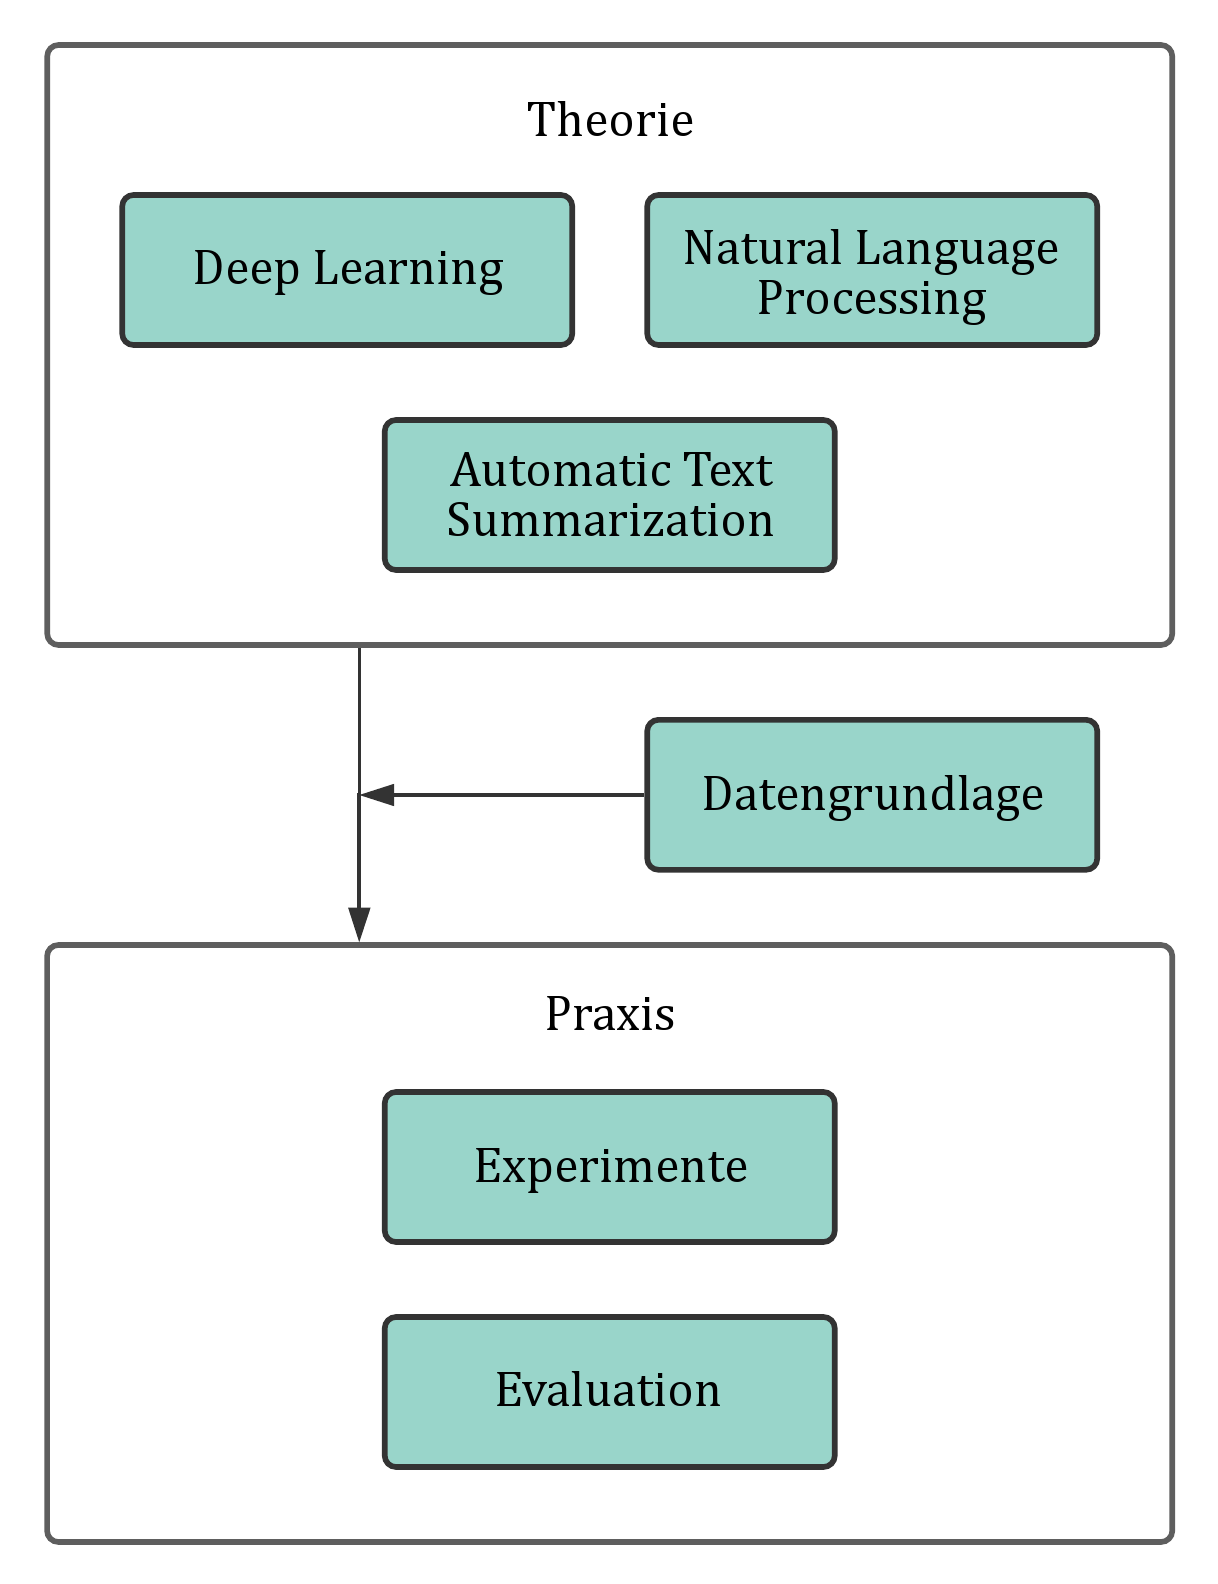
\includegraphics[width=0.55\linewidth]{./source/images/overview.png}}
  \caption{Aufbau der Arbeit.}
  \label{pic:Overview}
\end{figure}


\section{Forschungsstand \& Referenzen}
\noindent
Aufgrund der stetig fortschreitenden Entwicklungen überholt sich der Forschungsstand der \ac{ATS} regelmäßig. Dennoch haben sich in den vergangenen Jahren gewisse Tendenzen erkennen lassen. Bereits zur Jahrtausendwende existierten erste \ac{ATS}-Systeme. Waren die ersten Ansätze zumeist noch extraktiv, wurde sich in den vergangenen Jahren mehr und mehr auf die abstraktiven Ansätze konzentriert. Vor 2016 schienen Ansätze mit \ac{RNN} und \ac{LSTM} sehr populär \cite{NAL16}. In den Jahren 2016 und 2017 etablierten sich Ansätze, welche auf \ac{RL} basierten \cite{PAU17}. Seit 2018 legten diverse Ansätze mit Encoder-Decoder-Architekturen die Grundlage des heutigen \ac{SOTA} \cite{YAN19, ROT20}, denn um den \ac{SOTA} konkurrieren fast ausschließlich sogenannte Transformer. Diese basieren auf den Encoder-Decoder-Architekturen, implementieren verschiedenartige Attention-Mechanismen und haben sich sowohl unter qualitativen als auch unter ökonomischen und ökologischen Aspekten bewiesen \cite{ZHA20}. Diese Arbeit wird daher ebenfalls diesen Ansatz verfolgen, darüber hinaus jedoch die bislang unzulänglich behandelte Adaption auf die deutsche Sprache behandeln.\\

\noindent
Die Qualität der \ac{ATS} kann mithilfe des sogenannten ROUGE-Scores evaluiert werden. Dieser wird ebenso wie andere noch unerklärte Architekturen in einem nachfolgenden Kapitel dieser Arbeit umfangreich erläutert und kann zunächst als gegeben betrachtet werden. Die folgenden ROUGE-Scores können als zu reproduzierende Vergleichswerte verstanden werden: R-Recall: 15.96, R-Precision: 10.34, R-Measure: 12.22.\\

\noindent
Weiterhin hat der Durchbruch frei verfügbarer vortrainierter Modelle die \ac{NLP}-Welt revolutioniert, wie beispielsweise \ac{BERT} \cite{DEV19} sowie diverse Weiterentwicklungen. Verschiedenste \ac{NLP}-Aufgaben wie die \ac{ATS} konnten hiervon sehr stark profitieren. Die konkreten Funktionsweisen werden ebenfalls im Verlauf dieser Arbeit offengelegt. Wissenschaftliche Publikationen, welche mit dieser Arbeit vergleichbar sind und in dieser Arbeit oftmals referenziert werden, lauten wie folgt:

\begin{itemize}
	\item Text Summarization with Pre-Trained Encoders \cite{YAN19}
	\item German Abstractive Text Summarization using Deep Learning \cite{NIT19}
	\item Leveraging Pre-Trained Checkpoints for Sequence Generation \cite{ROT20}
\end{itemize}

\noindent
Eben genannte Informationen werden in einem entsprechenden Kapitel zur \ac{ATS} im Verlauf der Arbeit nochmal vertieft, wenn entsprechende Grundlagen kenntlich gemacht wurden. Dort werden der Forschungsstand und vergleichbaren Arbeiten separat thematisiert sowie entsprechende Verbesserungen hervorgehoben.
